\section{Grundlegende Architektur}\label{sec:architecture}

\begin{wrapfigure}{r}{0.5\columnwidth}
	\centering
	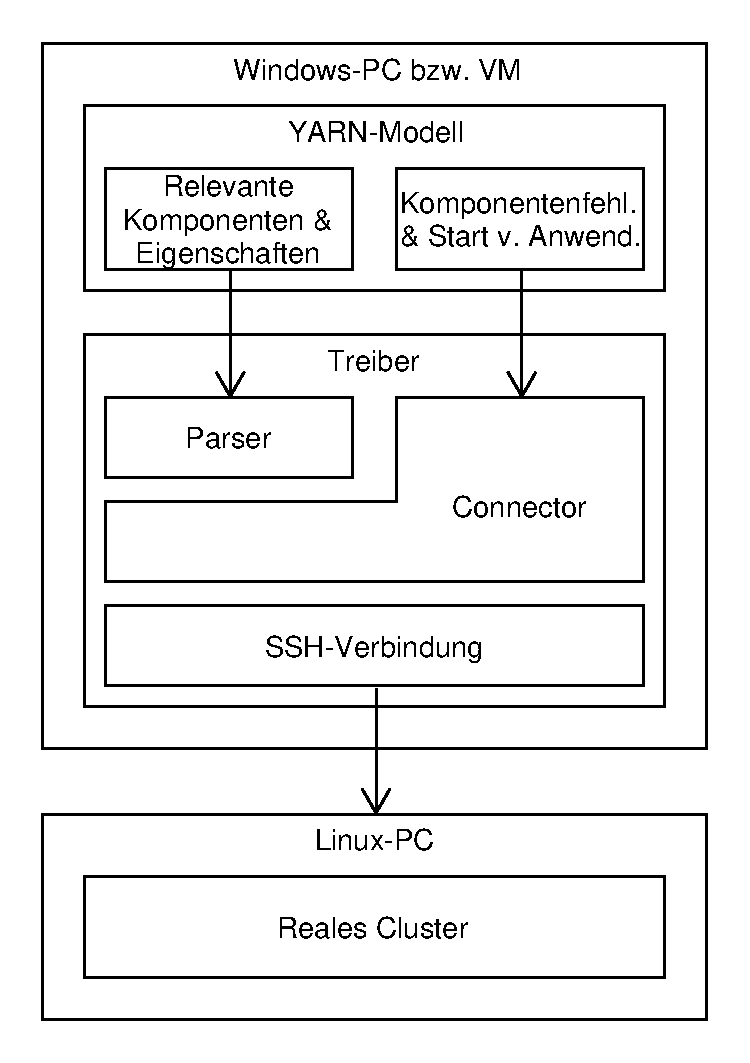
\includegraphics[width=0.5\columnwidth]{./images/modelArchitecture.pdf}
	\caption{Grundlegende Architektur des Gesamtmodells}
	\label{fig:modelArchitecture}
\end{wrapfigure}

Die grundlegende Architektur des gesamten Aufbaus besteht aus den drei in \autoref{fig:modelArchitecture} zu sehenden Schichten. Die oberste Schicht bildet dabei das \sS-Modell von Hadoop YARN, welches die wesentlichen YARN-Komponenten und dessen Komponentenfehler abbildet. Das reale Pendant dazu bildet das reale Cluster als unterste Schicht. Die Verbindung zwischen dem Modell und dem realen Cluster bildet der Treiber als eigenständige Schicht, bestehend aus den Kernkomponenten Parser, Connector und der eigentlichen SSH-Verbindung zum realen Cluster. Da \sS auf dem .NET-Framework aufbaut, ist für den \sS-MC entsprechend ein Windows dafür nötig, während das reale Cluster auf einem eigenen Linux-PC ausgeführt wird, weshalb als Konsequenz zur Kommunikation zwischen Modell und Cluster eine SSH-Verbindung nötig ist.